

\documentclass[twoside,twocolumn]{article}

\usepackage{blindtext} % Package to generate dummy text throughout this template 
\usepackage{graphicx}
\usepackage[sc]{mathpazo} % Use the Palatino font
\usepackage[T1]{fontenc} % Use 8-bit encoding that has 256 glyphs
\linespread{1.05} % Line spacing - Palatino needs more space between lines
\usepackage{microtype} % Slightly tweak font spacing for aesthetics

\usepackage[english]{babel} % Language hyphenation and typographical rules

\usepackage[hmarginratio=1:1,top=32mm,columnsep=20pt]{geometry} % Document margins
\usepackage[hang, small,labelfont=bf,up,textfont=it,up]{caption} % Custom captions under/above floats in tables or figures
\usepackage{booktabs} % Horizontal rules in tables

\usepackage{lettrine} % The lettrine is the first enlarged letter at the beginning of the text

\usepackage{enumitem} % Customized lists
\setlist[itemize]{noitemsep} % Make itemize lists more compact

\usepackage{abstract} % Allows abstract customization
\renewcommand{\abstractnamefont}{\normalfont\bfseries} % Set the "Abstract" text to bold
\renewcommand{\abstracttextfont}{\normalfont\small\itshape} % Set the abstract itself to small italic text

\usepackage{titlesec} % Allows customization of titles
\renewcommand\thesection{\Roman{section}} % Roman numerals for the sections
\renewcommand\thesubsection{\roman{subsection}} % roman numerals for subsections
\titleformat{\section}[block]{\large\scshape\centering}{\thesection.}{1em}{} % Change the look of the section titles
\titleformat{\subsection}[block]{\large}{\thesubsection.}{1em}{} % Change the look of the section titles

\usepackage{fancyhdr} % Headers and footers
\pagestyle{fancy} % All pages have headers and footers
\fancyhead{} % Blank out the default header
\fancyfoot{} % Blank out the default footer
\fancyhead[C]{Virtualizacion y contenedores $\bullet$ Mayo 2019 $\bullet$ } % Custom header text
\fancyfoot[RO,LE]{\thepage} % Custom footer text

\usepackage{titling} % Customizing the title section

\usepackage{hyperref} % For hyperlinks in the PDF

%----------------------------------------------------------------------------------------
%	TITLE SECTION
%----------------------------------------------------------------------------------------

\setlength{\droptitle}{-4\baselineskip} % Move the title up

\pretitle{\begin{center}\Huge\bfseries} % Article title formatting
\posttitle{\end{center}} % Article title closing formatting
\title{Virtualizacion y Contenedores} % Article title
\author{Andre Reinoso, Samuel Nuñez, Andres De la Barra ,David Damian y Richard Cruz Escalante}
\date{\today} % Leave empty to omit a date
\renewcommand{\maketitlehookd}{%
\begin{abstract}
\noindent The technologies are growing, extending and with this, new tools always appear to know and make use of them. In the present work we proposed to understand thoroughly the concepts of virtual machine and container and to make an analysis to both concepts. The result after the discussion is a critical appreciation of both concepts and a comparison to the context in which we find ourselves when using them.
\end{abstract}
}

%----------------------------------------------------------------------------------------

\begin{document}

% Print the title
\maketitle

%----------------------------------------------------------------------------------------
%	ARTICLE CONTENTS
%----------------------------------------------------------------------------------------

\section{Introduccion}

\lettrine[nindent=0em,lines=3]{L}a virtualización ha sido identificada como una de las diez tecnologías estratégicas en el año 2010. Consiste en la extracción del software de una computadora, encapsulándolo en algo que llamaremos máquina virtual, que será ejecutada en una máquina física ajena a la anterior.
Años después surgieron los contenedores, son la vía que nos coloca Docker para tener el mismo uso que con las maquinas virtuales creadas de la forma tradicional. Docker utiliza estos contenedores para aislar uno o más procesos. Estos procesos en el Host necesitan Memoria, CPU, Acceso a la Red y espacio en disco. Es un ambiente perfecto para que las aplicaciones puedes funcionar de forma correcta.
En el presente trabajo se definirán los conceptos de maquina virtual, contenedores y se tratara el tema de la diferencia entre ambos.



%------------------------------------------------

\section{Objetivos}

\begin{itemize}
\item Entender qué es una máquina virtual.
\item Entender qué es un contenedor.
\item Comparar ambos conceptos.
\item Establecer un juicio acerca de las ofertas y el potencial de ambas.

\end{itemize}




%------------------------------------------------

\section{Desarrollo}

\subsection{¿Que es una maquina virtual?}

Una máquina virtual es un software que emula un ordenador justo como si fuese uno real. Todo esto sucede en una ventana dentro de tu sistema operativo actual como cualquier otro programa que uses. La idea de este tipo de software es que puedas ejecutar sistemas operativos como si fuesen una aplicación, mientras este cree que está usando el hardware de un ordenador físico común. Cada vez que quieras usar este sistema operativo puedes abrir el software de virtualización y «encender» tu máquina.
Un sistema de virtualización debe ser capaz de ofrecer una interfaz en la máquina anfitriona para poder interactuar con el sistema operativo de la máquina virtual. Además, la máquina anfitriona debe ofrecer una interfaz de sus recursos a la máquina virtual para que pueda utilizarlos. De estas interfaces de comunicación se encarga un software que se instala en la máquina anfitriona para poder ejecutar las máquinas virtuales. Existen muchos tipos de software de virtualización en el mercado, tanto software propietario como software libre y para ejecutarse sobre máquinas anfitrionas que funcionen como servidores, o bien sobre cualquier computadora personal. Entre los más utilizados están VirtualBox y Virtual PC para computadoras personales, Xen y KVM para servidor, y VMware para ambos. (Martin, 2011)

Lo que sucede es que se ejecuta en una ventana, igual que cualquier otro programa, y permite que el usuario final tenga la misma experiencia en una máquina virtual que tendría en el propio sistema operativo host. La máquina virtual se sitúa en un espacio aislado del resto del sistema, es decir, el software de la máquina virtual no puede interferir con el equipo en sí. Esto crea un entorno ideal para probar otros sistemas operativos, incluidas versiones beta, acceder a datos infectados por virus, crear copias de seguridad de sistemas operativos y ejecutar software o aplicaciones en sistemas operativos para los que no se habían creado inicialmente.
Se pueden ejecutar varias máquinas virtuales a la vez en un mismo equipo físico. Para servidores, los diversos sistemas operativos se ejecutan en paralelo con un fragmento de software denominado hipervisor para administrarlos, mientras que los equipos de escritorio suelen implementar un solo sistema operativo para ejecutar los demás sistemas operativos en ventanas de programa. Cada máquina virtual proporciona su propio hardware virtual, incluidas las CPU, memoria, unidades de disco duro, interfaces de red y otros dispositivos. El hardware virtual se asigna después al hardware real de la máquina física, lo que permite ahorrar costos, porque reduce la necesidad de tener sistemas de hardware físico, con los costos de mantenimiento que conllevan, y también reduce la demanda de alimentación y refrigeración.

\begin{center}
	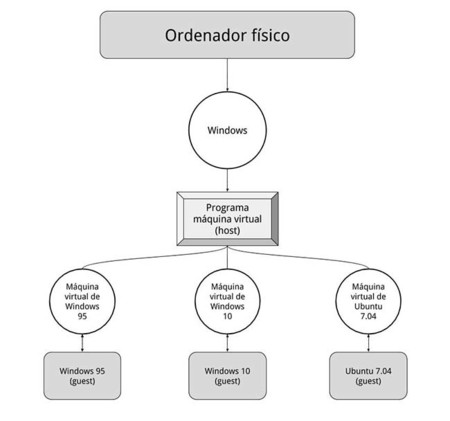
\includegraphics[width=5cm]{./Imagenes/virtualizacion} 
	\end{center}




\subsection{¿Que es un contenedor?}

Los contenedores son aplicaciones y servicios autónomos que encapsulan todas las dependencias para que sean fácilmente implementables y actualizables.\\
Los contenedores son aplicaciones independientes, empaquetadas con sus dependencias.\\
Los contenedores se distribuyen fácilmente a través de una plataforma virtual.

\begin{itemize}
\item Docker
\\ Éste contenedor empaqueta todo lo necesario para que uno o más procesos (servicios o
aplicaciones) funcionen: código, herramientas del sistema, bibliotecas del sistema, dependencias,
etc.
\\Usos de Docker
\\Ya que los contenedores te dan un ambiente aislado del resto del sistema, las posibilidades de
trabajo incluyen
\\ \textbf{- Empaquetamiento y despliegue de aplicaciones automatizado y controlado}
\\ \textbf{- Creación Ambientes de PaaS.}
\\ \textbf{- Testing e integración continua}
\\ \textbf{- Despliegue y escalamiento de aplicaciones y bases de datos.}

\begin{center}
	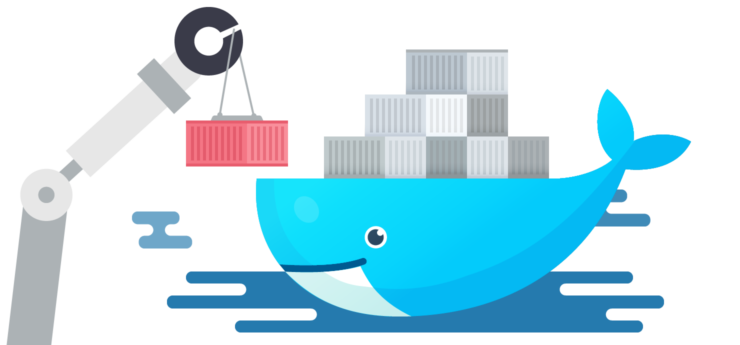
\includegraphics[width=5cm]{./Imagenes/docker} 
	\end{center}

Ventajas
\\ \textbf{- Las instancias se inician en pocos segundos.}
\\ \textbf{- Son fácilmente replicables.}
\\ \textbf{- Es fácil de automatizar y de integrar en entornos de integración continua.}
\\ \textbf{- Consumen menos recursos que las máquinas virtuales tradicionales.}
\\ \textbf{- Ocupan mucho menos espacio.}
\\ \textbf{-Permite aislar las dependencias de una aplicación de las instaladas en el host.}

Desventajas
\\ \textbf{- Sólo puede usarse de forma nativa en entornos Unix con Kernel igual o superior a 3.8.}
\\ \textbf{- Sólo soporta arquitecturas de 64 bits.}
\\ \textbf{- Como es relativamente nuevo, puede haber errores de código entre versiones.}
\end{itemize} 

\subsection{¿Diferencia entre maquinas virtuales y contenedores?}
El objetivo principal de estas tecnologias, es la de dar un entorno de desarrollo con ciertas caracteristicas por lo que parecen estas tecnologias, maquinas virtuales y contenedores, donde la primera es una copia exacta del software y hardware, en cambio los contenedores no hay una copia si no que tienen los archivos necesarios para poder correr un determinado software.

\begin{itemize}
	\item Jerarquia maquina virtual
	\\La primer gran diferencia es la jerarquia, forma de como estan constituidas. En el primero de los casos las maquinas virtuales estan constituidas por:
	\\ \textbf{-El servidor o una computador}.
	\\ \textbf{-El sistema operativo} que hospeda y administra los recursos del servidor o computador.
	\\ \textbf{-El hypervisor} plataforma que monitoriea y controlas virtualizacion.
	\\ \textbf{-Sistema virtualizado} sistema operativo que fue virtualizado (copia total de software y hardware).
	\\ \textbf{-Bins/Libs} Binarios y librerias.
	\\ \textbf{-App} Aplicacion a ejecutar.
	\begin{center}
	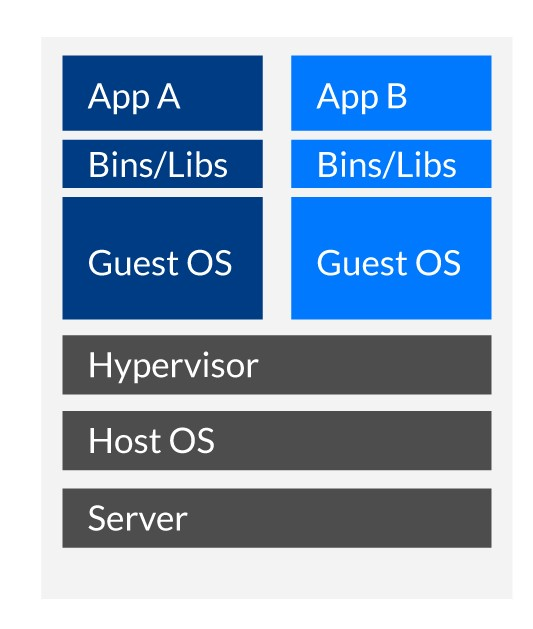
\includegraphics[width=5cm]{./Imagenes/jerarquia1} 
	\end{center}
\end{itemize} 

\begin{itemize}
	\item Jerarquia contenedor
	\\ \textbf{-El servidor o una computador}.
	\\ \textbf{-El sistema operativo} que hospeda y administra los recursos del servidor o computador.
	\\ \textbf{-Docker Engine} virtualizacion a nivel del sistema operativo permite multiples instancias aisladas.
	\\ \textbf{-Bins/Libs} Binarios y librerias.
	\\ \textbf{-App} Aplicacion a ejecutar.
	\begin{center}
	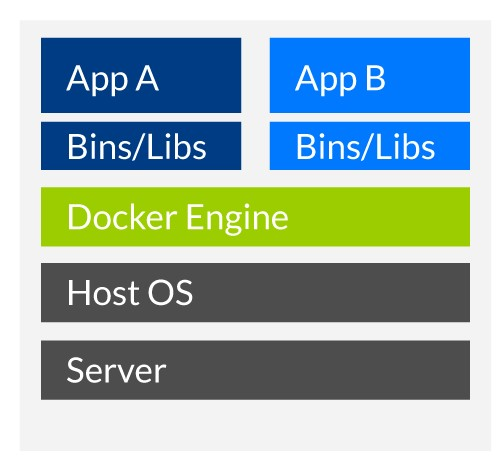
\includegraphics[width=5cm]{./Imagenes/jerarquia2} 
	\end{center}
\end{itemize} 

\begin{itemize}
	\item Los contenedores permiten desplegar aplicaciones más rápido, arrancarlas y pararlas más rápido y aprovechar mejor los recursos de hardware.
	\item La solución de virtualización permite gestionar de forma centralizada los sistemas virtualizados así como sus recursos de almacenamiento:
	\item Reducción de los costes de IT gracias al aumento de la eficiencia y la flexibilidad en el uso de recursos.
	\item Administración global centralizada y simplificada.
	\item Mejora en los procesos de clonación y copia de sistemas: Mayor facilidad para la creación de entornos de test que permiten poner en marcha nuevas aplicaciones sin impactar a la producción, agilizando el proceso de las pruebas.
	\item Aislamiento : un fallo general de sistema de una máquina virtual no afecta al resto de máquinas virtuales.



\end{itemize} 

\section{Conclusiones}

Para hablar de contenedores y virtualizadores, era necesario observar el crecimiento de las tecnologías y el cómo se han ido extendiendo. Cuanto más plataformas, cuantas más librerías, es más compleja la unificación de los recursos para el despliegue de una aplicación en todas las distribuciones. Con esto apareció el concepto de máquina virtual, que pretendió hacerle frente a esta brecha tecnológica, pero más adelante aparecería otro concepto más, que es el de los contenedores, y que buscan responder directamente a la primera necesidad del usuario: el despligue de su aplicación.
Mientras que el enfoque de la virtualización es la de levantar un sistema operativo entero montado en una máquina virtual para su uso, la idea del contenedor es de proveer de las librerías necesarias para el levantamiento de la aplicación en sí, lo cual suena más provechoso para su uso pues esta última propuesta ofrece muchas ventajas. Sin embargo, creemos que ambos conceptos tienen buenas garantías qué ofrecer y la recurrencia de cualquiera de las dos queda siempre quedará en primer lugar referido a la necesidad del usuario y de lo que esté buscando. Entonces a pesar de que existan muchas diferencias entre ambos conceptos, viéndolo desde la perspectiva de la necesidad, ninguno de los dos conceptos no se desbaratarían.
%----------------------------------------------------------------------------------------
%	REFERENCE LIST
%----------------------------------------------------------------------------------------

\begin{thebibliography}{99} % Bibliography - this is intentionally simple in this template

\bibitem[Martin, 2011]{Diego Martin:2011dg}
Martin, M.M,  y J.U (2011).
\newblock Virtualización, una solución para la eficiencia,
seguridad y administración de intranets
\newblock {\em El profesional de la informacion}, 350.
\newblock Contenedor de aplicaciones: Docker (2015)
 
 
\end{thebibliography}

%----------------------------------------------------------------------------------------

\end{document}
